\section{Neural network implementation and models}
Building neural network for classifying pain maps was trial and error process.
In this project the deep learning method is used to classify the pain maps and gender by determined outputs. The data is a set of 2D-images combined with gender and the outputs are pain intensity and duration. For classification purpose supervised convolutional neural network is used followed by fully-connected layers at the end. This architecture of the model is chosen to the interest of morphology and location of the pain. The models are trained, and tested on a single computer with GPU and ran on Python programming language with Keras library. Specifications of hardware and software are described in detail in \autoref{sec:softHard}.

\subsection{Software and hardware}\label{sec:softHard}
The neural network developed for this study, was programmed using Python v3.6.3. Python is an object-oriented and general-purpose programming and scripting language, that may be used for e.g. programming websites, mobile applications, but also for machine learning programming applications.
For development of deep learning application in python, different libraries are available, where some of the popular are the Theano and TensorFlow libraries.\citep{Swamynathan2017}. The Tensorflow v1.3.0 library was chosen for this study. %TensorFlow is an open source library for development of machine learning applications, that has been released by Google \citep{Swamynathan2017}.  
An additional library, Keras v2.0.8, was imported, which runs on top of either Tensorflow or Theano, and is a high-level neural networks application programming interface (API).   
Keras is a simplified version of the two libraries, which allows for fast and easier prototyping of neural network \citep{Chollet2015}. This was deemed suitable given that no previous experience with neural network were available during this study.  

Utilization of graphics processing unit (GPU) computation was also implemented using CUDA drivers and cnDNN communication libraries, which allowed for faster runtimes, then through the use of the central processing unit (CPU).
 
%Keras is a simplified version of the two libraries, which makes it easier to program in Python, but still allows for building complex models. TensorFlow is an open source library for development of machine learning applications, that has been released by Google \citep{Swamynathan2017}. 
%Using CPU or GPU on this platform the most mathematical operation  is computed in a computerized and simple way \citep{Swamynathan2017}. A small example of the concept of using TensorFlow could be seen in Appendix B. The plots for this model are generated using Tensorboard visualizing tool. It allows to watch a graph during the training, gives plot quantitative metrics and shows data like images that pass through it. Besides visualizing part of this tool it is also useful for debugging as it allows to observe the graph at a present time.\citep{Abadi2016a}

\noindent
The neural network was developed on a laptop with 4x 'Intel® Core™ i7' CPU‘s and one GPU of type 'Geforce GTX 970M' with specifications listed in table \ref{tab:Specs}.

%\begin{figure} [H]
%\centering
%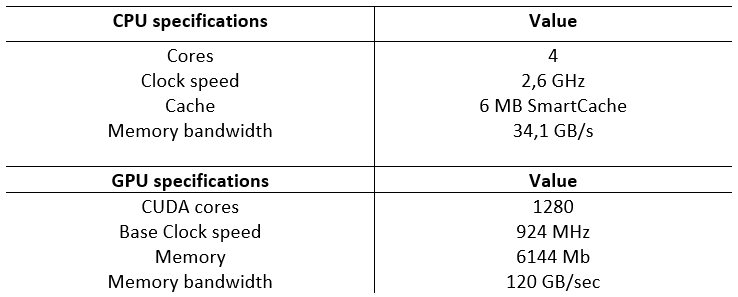
\includegraphics[width=1\textwidth]{figures/Specs}
%\caption{Specifications of CPU‘s and GPU \citep{Intel,Nvidia}.}
%\label{tab:Specs}
%\end{figure}

\begin{table}[H]
\centering
\begin{tabular}{p{4cm}|p{4cm}}
\hline
CPU specifications &  Value \\ \hline
Cores & 4 \\
Clock speed & 2.6 GHz \\ 
Cache & 6 MB SmartCache  \\ 
Memory bandwidth & 34.1 GB/s \\ \hline
GPU specification & Value \\ \hline
CUDA cores & 1280  \\
Base Clock speed & 924 MHz  \\
Memory & 6144 MB  \\
Memory bandwidth & 120 GB/s  \\ \hline
\end{tabular}
\caption{Specifications of CPU and GPU \citep{Intel,Nvidia}}
\label{tab:Specs}
\end{table}

\subsection{Data handling and design choices of the models}
This section presents the different models, their architecture and implementation used in this study.
For classification of each representation a corresponding model was made. The classifier models for \textit{morphology-} and \textit{combined-} representation were operating on a pixel level by learning features of the pain charts, whilst the \textit{location} representation operated from the 10 element location vector. 
The architecture of the models consist two main parts, a convolution part and a fully-connected part, except the \textit{location} model that only consist of the latter.   
Convolution works as feature extraction of the pain maps, where convolutional and pooling layers alternates in order to extract relevant features out of the image, as described in \autoref{sec:Layers}.
The fully-connected part works as classification, where computed feature maps gets weighted and classified to a particular class in the output layer. 
A higher generalization performance of the classifiers, was investigated through the use of regulation and optimization methods.
The available data was separated into a training and test subset, from which training data was used to regulate and optimize the model. 
Supervised learning was used for training the three models. The common input for all of the model were gender, along with the different image representation

%, as presented in figure \ref{fig:schema1}. 
% These inputs are trained and then compared against their respective category label. 

%From the higher point of view, the model can be architecturally split into two main parts. Feature extraction part, where convolutional and pooling layers alternates in order to extract the most important features out of the image. Second part is called classification, where computed feature maps will be assigned to particular class of the output layer. In order to obtain a higher generalization performance of deep learning classifier, methods like activation function, regulation and optimization will be used within the layers were implemented into the models.

\subsubsection{Location-representation model}
Given the location representations relative simplicity, in the form of a 11 element row-vector that contains both the pain maps information along with a gender value as described in \ref{sec:Regions} , the architecture of the model is also relatively simple, compared to the other models.  
For this representation the model consists of four fully-connected layers where the last of the layers is the output layer, where the number of outputs matches the number of classes. 
It was chosen not to use convolution layers, like in the morphology- and combined-representation, because it was believed that be no greater benefit given how convolution works, and the size of the location representation. 
An overview of the architecture of the model for the location representation can be seen in \ref{fig:Simpleschema}.

\begin{figure} [H]
\centering
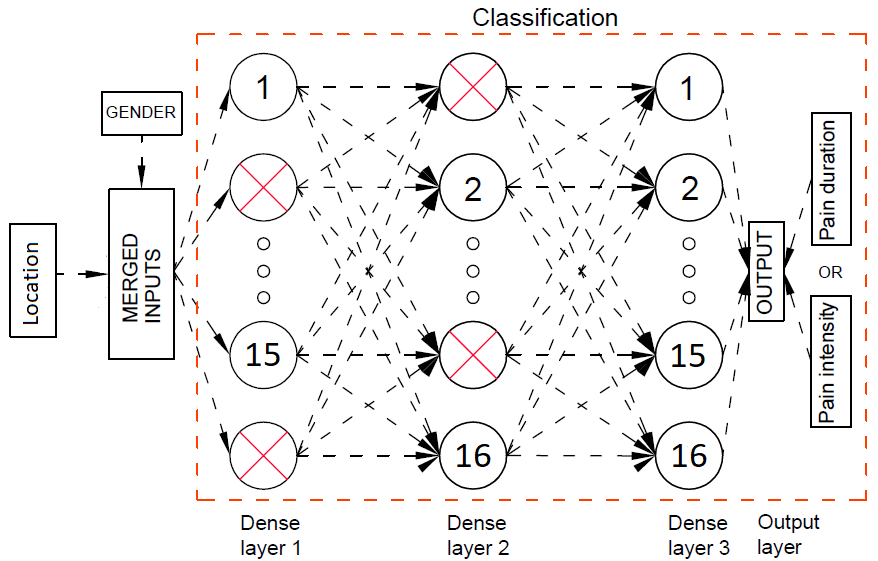
\includegraphics[width=0.6\textwidth]{figures/Simpleschema}
\caption{Architecture of the location-representation model.}
\label{fig:Simpleschema} 
\end{figure}


\subsubsection{Morphology-representation model}
The models for the morphology representation, consists of convolution, maxpooling and fully-connected layers.  
The models are essentially made up of two parts, where one being the extraction of image features, and another being a classification part. 
For the extraction of image features a series of three convolution and maxpooling layer are stacked after each other, to which the first layer is specified to receive the main input of the shape $1 \times 118 \times 252$ where the 1 reflects the fact that the pain map representation is binary. 
The classification part of the network is the same architecture as that of the model for the location representation, and thereby consists of fully-connected layers. Between these two parts of the model, a secondary input is added specifying the gender related to the given pain map. 
Before the pain maps features reach the fully connected layers it is flattened from the shape of a matrix to that of a single row in order to merge the extracted features with gender. The merged data passes through fully connected layers and reaches the output layer where it is given a percentage value according to which class it fits the most. 
The architecture of the morphology representation model is shown in figure \ref{fig:Schema1}.

\begin{figure} [H]
\centering
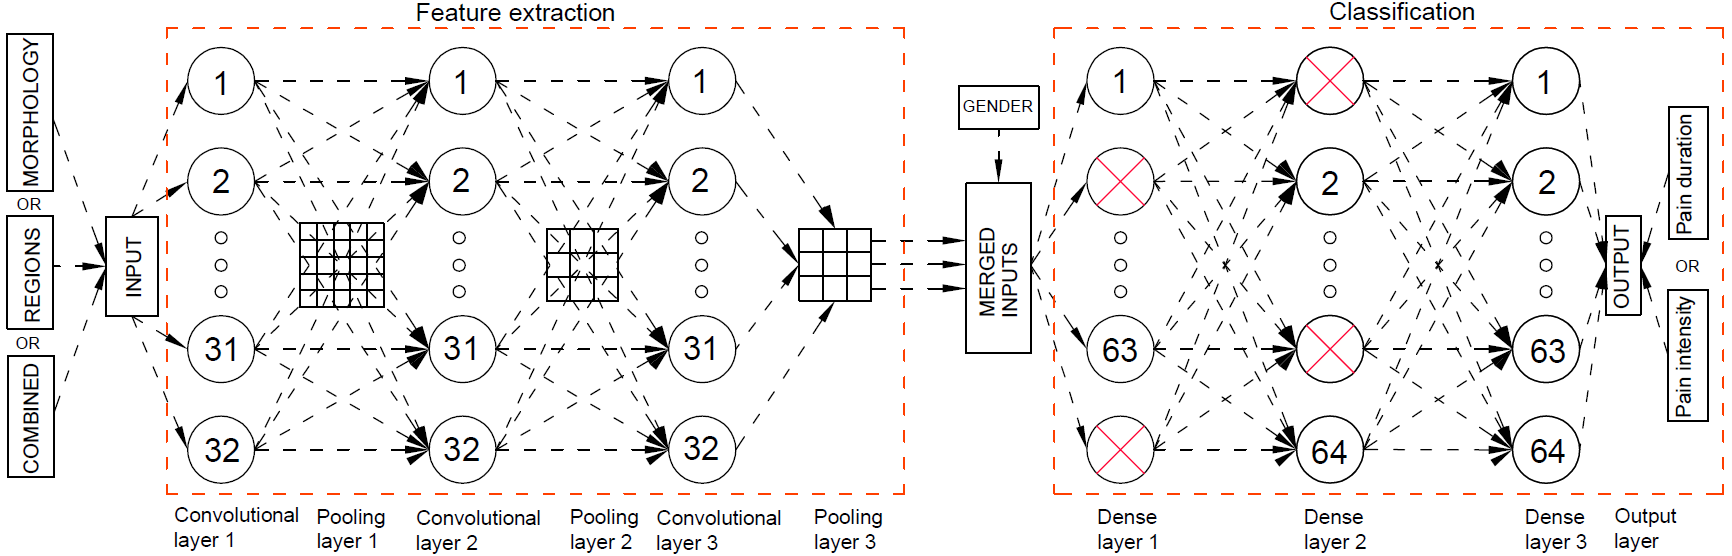
\includegraphics[width=1.0\textwidth]{figures/Schema1}
\caption{Architecture of the neural network model used for this study.}
\label{fig:Schema1} 
\end{figure}



\subsubsection{Combined-representation model}
The architecture of this model is nearly identical to that of the morphology representation model, as seen in \autoref{fig:Schema1}. 
The main difference can only be seen in the dimension of input for the pain map representation, where the input shape is $10 \times 118 \times 252$ to which 10 is the number of image layers per. pain map. This is the result of the one-hot encoding done to the images as described in \ref{sec:combined}. 


\subsection{Data handling in python}
Pre-processed data is loaded from a \textit{.mat} file into python.
Data within the file was pre-shuffled and split into a training and test subsets, as described in \autoref{sec:prepros}. The training subset was made up 85\% of the available data and test subset the remaining 15\%. Data was pre-shuffled to ensure that the training and test subset were separated at random. Furthermore the data was separated to prevent data used for training to be used for testing, to which this would give a false estimation of performance.  
%In Python the training subset is further divided into a training and validation subsets. 
The training subset was used to train and optimize the models, to find the optimal weights with the back-propagation algorithm \citep{Bengio2012}. 
The test subset was used to evaluate the generalization of the model, after training and optimization.
Morphology, and combined representations, were reshaped from a row vector, back into a matrix to retain their 2D structure of the pain map.
Classification labels used for during supervised learning was one-hot encoded, so the number of label values were compatible to the number of outputs in the models. This was a result of the loss function \textit{categorical\_crossentropy} used for the models, that tries to reduce loss between the categories.    


\section{Optimization}
To reduce overfitting and improve general performance of the model, different methods was tested and implemented. 
The performance of the models was evaluated from an average accuracy, sensitivity and specificity, that was calculated from a 10-fold cross validation on the training subset. s
A grid search method was used to find optimal hyperparameters for the models. This allowed to run the models through different parameters, from which the parameters the resulted in the highest performance was used.  by cross-validating them 5 times and evaluating the mean values with SD. Activation function, dropout, optimizer, learning rate, type of initializer, number of neurons, batch size and number of epochs were tested using this method.  All used optimization techniques are presented in this section and table with used values is presented in FIGURE or RESULTS section (x,x)

\subsubsection{Activation function}
For all models the activation function in all layers except the output layer was the ReLu function. This was chosen as this is seen as the most common activation function in more modern neural networks. The reason for it's popularity is that it prevents the problem known as the vanishing or exploding gradient, typically seen when using sigmoid activation function i the hidden layer. \citep{Goodfellow2016}    
%During this study different activation functions, such as ReLu, Softmax, Sigmoid were tested. Results were compared using grid-search and ReLu was picked as activation function for the models. Activation function was implemented in convolutional and fully-connected layers. 
Sigmoid activator was used for final output layer, because.

\subsubsection{Dropout}
Dropout is implemented in the models due to the benefits described in section \ref{sec:dropout}. Dropout of three different values were tested on grid-search and 0.5 were picked as it scored the highest. This regulator is only used within the hidden fully-connected layers, where it is defined to randomly drop 50 \% of the nodes. Dropout is shown in figure \ref{fig:Simpleschema} and marked as red crosses. 

\subsubsection{Optimizer}
Adam, RMSprop, Adagrad and SGD, presented in section \ref{sec:optimizers}, were tested and compared. SGD scored the highest and was implemented while compiling the model.

\subsubsection{Learning rate}
In order to determine the most optimal \textit{learning\_rate} for the Adam  and SGD optimizers several different values were tested. Default value 0,001 performed higher than values of 0,01 and 0,0001. To fit the model this parameter was set to 0,001 meaning that the convergence of gradient descent is reached slower but with more accurate \textit{minima}. 

\subsubsection{Batch size and number of epochs}
Three different values of batch size and number of epochs were chosen based on computing power. Grid search on batch size were tested on 5, 10, 15 values, while number of epochs were 15, 25, 35. On every data representations these hyperparameters varied. Batch size and number of epochs were used during the fit process.

\subsubsection{Weight and biases initializing}
Weights and biases initialization was performed, since it affects the performance of the model.
A grid search of weight initializer using \textit{uniform}, \textit{lecun\_uniform}, \textit{normal}, \textit{glorot\_normal} and \textit{glorot\_uniform} were tested and results revealed that \textit{glorot\_normal} performed the best by 3,2 \% compared to the second best. Results can be seen in \ref{pictureFromCMD}. Weight initializer was used in convolutional and fully-connected layers.
Biases were initialized to zeros values
% See image - kernal_init.png 

\subsubsection{Number of neurons}
Number of neurons were chosen based on the best performance comparing 16, 32, and 64 neurons per hidden layer. 32 in convolutionals and 64 neurons in fully-connected layers scored the highest in terms of accuracy. These values were used in in the model within all data representations.

\subsection{Training and validation}
The training was performed using mini-batches of size 10 with SGD optimizer with default learning rate, explained in section \ref{sec:optimizers}. Data was split into train(75\%), validation (15\%), and test (10\%) sets, and the models were regularized using dropout (50\%). Number of neurons in hidden layers were decided to be used as 32 for convolutional and 64 for fully-connected layers. All networks were using ReLu activation function, except output layers, which were using Sigmoid activator instead, described in Section %{activation function}.
The model weight parameters were initialized at random values using \textit{glorot\_normal}, biases parameters were initialized to zero values.

\subsubsection{Stratified m-folds cross-validation}
As a result of binary output, 10-fold cross-validation method were used for training the data and evaluating the performance of the models. Folds were separated 10 times randomly in relation to the distribution of the classes. Stratified m-folding prevents the fold to contain the data of one class. Accuracy, sensitivity and specificity were calculated after each fold and the mean values of these parameters were generated at the end of the training. Results are given in section %{the results}.

\subsubsection{Error and accuracy graphs)}
During each training and validating epoch, the error and accuracy is calculated and presented as graph at the end. According the error graph, the overfitting or underfitting could be determined. Model could be optimized based on these results with technique described in section \ref{sec:optimizers}.

\subsection{Testing}
The testing or prediction refers the generalization performance from the given classification question and is the main job for the neural network.
Separated 10\% dataset were used for testing how accurate the training model can perform using unknown data. By feeding new data into the network, testing process begins. At each time-step classifier predicts the probability for every possible class, and selects with the highest probability as it prediction, giving it as a percentage result. Predictions were presented as a confusion matrix in section {results} providing true positive and negative together with false positive and negative results.
